%\documentclass[a5paper,headsepline,titlepage,11pt,nnormalheadings,DIVcalc]{scrbook}
\documentclass[a5paper,headsepline,titlepage,11pt,nnormalheadings,DIVcalc]{book}
\usepackage[a5paper,backref]{hyperref}
\usepackage[papersize={165mm,215mm},twoside,bindingoffset=0.5cm,hmargin={2cm,2cm},
				vmargin={2cm,2cm},footskip=1.1cm,driver=dvipdfm]{geometry}
%\usepackage[papersize={148mm,215mm},twoside,bindingoffset=0.5cm,hmargin={2cm,2cm},
%				vmargin={2cm,2cm},driver=dvipdfm]{geometry}
%\usepackage{palatino}
\usepackage{graphicx}
\usepackage{wrapfig}
\usepackage[bahasa]{babel}
\usepackage{fancyhdr}
\usepackage{longtable}
\usepackage{hhline,multirow}
\usepackage{pst-node}

%\setlength{\voffset}{0.5in}
%\setlength{\oddsidemargin}{28pt}
%\setlength{\evensidemargin}{0pt}
\renewcommand{\footrulewidth}{0.5pt}
\lhead[\fancyplain{}{\thepage}]%
      {\fancyplain{}{~}}
\rhead[\fancyplain{}{~}]%
      {\fancyplain{}{\thepage}}
\pagestyle{fancy}
\lfoot[\emph{Informasi 2010}]{}
\rfoot[]{\emph{Lingkungan St Petrus Maguwo}}
\cfoot{}

\newcommand{\BU}[1]{\begin{itemize} \item[U:] #1 \end{itemize}}
\newcommand{\BI}[1]{\begin{itemize} \item[I:] #1 \end{itemize}}
\newcommand{\BP}[1]{\begin{itemize} \item[P:] #1 \end{itemize}}
\title{Informasi Lingkungan St. Petrus}
\author{Wilayah Yohanes De Britto \\Stasi Maguwo \\Paroki Kalasan}
\date{2010}
\hyphenation{sa-u-da-ra-ku}
\hyphenation{ke-ri-ngat}
\hyphenation{je-ri-tan}
\hyphenation{hu-bung-an}
\hyphenation{me-nya-dari}
\hyphenation{Eng-kau}
\hyphenation{ke-sa-lah-an}
\hyphenation{ba-gai-ma-na}
\hyphenation{Tu-han}
\hyphenation{di-per-ca-ya-kan}
\hyphenation{men-ja-uh-kan}
\hyphenation{bu-kan-lah}
\hyphenation{per-sa-tu-kan-lah}
\hyphenation{ma-khluk}
\hyphenation{Sem-buh-kan-lah}
\hyphenation{ja-lan}
\hyphenation{mem-bu-tuh-kan}
\hyphenation{be-ri-kan-lah}
\hyphenation{me-ra-sa-kan}
\hyphenation{te-man-ilah}
\hyphenation{mem-bi-ngung-kan}
\hyphenation{di-ka-gum-i}
\hyphenation{ta-ngis-an-Mu}
\hyphenation{mi-lik-ilah}

\renewcommand*\thesection{\arabic{section}.}
\setlength{\parindent}{0mm} 

\begin{document}
\thispagestyle{empty}
%\maketitle
\newsavebox\IBox
%\sbox\IBox{\includegraphics[scale=0.4]{Saint-Peter-Apostle-e.eps}}

%% \psset{unit=1in}
%% \begin{pspicture}(4in,6.0in)
%% % set up the fonts we use
%% \DeclareFixedFont{\PT}{T1}{ppl}{b}{it}{0.4in}
%% \DeclareFixedFont{\PTsmall}{T1}{ppl}{b}{it}{0.3in}
%% \DeclareFixedFont{\PTsmallest}{T1}{ppl}{b}{it}{0.2in}
%% \DeclareFixedFont{\PTtext}{T1}{ppl}{b}{it}{11pt}
%% \DeclareFixedFont{\Logo}{T1}{pbk}{m}{n}{0.2in}
%% % place the front cover picture
%% \rput[cb](2.3,2.5){\usebox\IBox}
%% % put the text on the front cover
%% \rput[cb](2.5,5.3){\PT {Informasi}}
%% \rput[cb](2.5,4.8){\PT {Lingkungan St. Petrus}}
%% \rput[cb](2.5,0.6){\PTsmallest {Wilayah Yohanes de Britto}}
%% \rput[cb](2.5,0.3){\PTsmallest {Stasi Maguwo}}
%% \rput[cb](2.5,0.0){\PTsmallest {Paroki Marganingsih Kalasan }}
%% 
%% %\rput[cb](3,-1){\PTsmallest {\namagereja}} 
%% 
%% \end{pspicture}
%\tableofcontents 

\setlength{\parskip}{2mm}
\section*{Sejarah singkat Lingkungan St Petrus}
Lingkungan Santo Petrus yang ada sekarang ini (2010) sudah melewatai banyak liku-liku. Pada awalnya, yauitu tahun 1984, bernama Kring Santo Petrus yang meliputi dusun Nanggulan, Kopenrejo, Gondangan, Setan, Dewan, Kalongan,  dan Kembang. Kepengurusan periode awal ini diketuai oleh Ig. Mulyono yang diberkati oleh Rm Y. Suyadi, Pr, romo paroki Kalasan saat itu. Kepengurusan ini berakhir pada tahun 1987.

Periode berikutnya 1987-1990 Kring St Petrus memiliki umat sebanyak 159 warga dalam 53 keluarga dan sebagai ketua kring adalah Th Sukamto. 
%Peristiwa penting dalam periode ini adalah peresmian Gereja Bunda Maria oleh Uskup Agung Mgr. Y. Darmoatmojo SJ pada 2 Juni 1988. Selain itu pada tanggal 10 Oktober 1989 ada kunjungan Sri Paus Yohanes Paulus II di Yogyakarta. Gereja Bunda Maria mendapat kenang-kenangan berupa karpet merah sepanjang 25 m yang pernah dilalui oleh Sri Paus saat misa akbar di Adisucipto.
Pada penyerahan kepengurusan dari periode sebelumnya, H. Siswanto sebagai ketua lingkungan periode 1990-1993 menerima data jumlah umat lingkungan St Petrus sudah berkembang menjadi 71 keluarga yang terdiri atas 213 warga. Perubahan dari kring menjadi lingkungan sesuai dengan perubahan Wilayah Maguwo menjadi Stasi Maguwo pada tahun 1990. 
%Saat kepengurusan H. Siswanto ini terjadi mutasi 4 keluarga dengan 12 warga masuk dan 1 keluarga dengan 3 warga keluar. 
Mengingat wilayah St Petrus yang luas maka sesuai dengan kesepakatan dilakukan pemekaran menjadi 2 lingkungan yaitu St Petrus dan St Paulus. Lingkungan St Petrus meliputi Kembang, Nanggulan, Gondangan, Tajem, Setan, Karang Nongko, Sopalan. Lingkungan Paulus meliputi Rejoinangun, Dewan, Kalongan, Corongan.

Periode berikutnya 1993-1995 umat lingkungan mencapai 58 keluarga terdiri atas 223 warga dengan ketua T. Sukijo. Periode 1996-2001 ketua lingkungan dijabat oleh V. Sukiyanto dengan umat sejumlah 256 warga dalam 69 keluarga. Saat ketua dijabat oleh Y. Samin (2002-2004) umat berkembang menjadi 76 keluarga dengan 270 warga.

Wilayah Lingkungan St Petrus masih dirasa terlalu luas maka pada tahun 2006 saat kepengurusan FX Radjijo (2005-2007) dilakukan pemekaran lagi menjadi 2 lingkungan yaitu St Petrus dan St Fransiskus Asisi. Kedua wilayah dibatasi oleh {\it ring road}. 

Periode transisi 2006-2007 lingkungan St Petrus diketuai oleh Y.Z. Budiman S dengan umat sebanyak 162 dalam 48 keluarga. Saat ini lingkungan St Petrus mempunyai umat sebanyak 187 dalam 63 keluarga dan diketuai oleh V. Agung Danan Jaya.
 
\chapter*{Informasi Umat}

\section[Pengurus]{Pengurus lingkungan}

\subsection{Periode 2014 -- 2016}

%\footnotesize 
\begin{center}
SUSUNAN PENGURUS LINGKUNGAN SANTA THERESIA 
\par
PERODE TAHUN 2014 -- 2016
\end{center}

\begin{longtable}{p{0.5cm}p{4cm}p{5cm}p{4cm}}
\multicolumn{2}{l}{Ketua I}&Antonius Supriyana &+6285 865 355 895\\
\multicolumn{2}{l}{Ketua II}&FX. Sularto &+6281 314 190 698\\
\multicolumn{2}{l}{Sekretaris I}&Anastasi Bare &+6285 643 173 281\\
\multicolumn{2}{l}{Sekretaris II}&FX. Ari Wibowo Sudaryanto&+6285 8633 5678\\
\multicolumn{2}{l}{Bendahara I}&Theresia Prima Ari Setiyani&+6285 6288 6539\\
\multicolumn{2}{l}{Bendahara II}&Agnes Sukarmi&+6281 328 795 814\\

\setcounter{nourut}{0}\\
\multicolumn{2}{l}{\textit{\textbf{Tim Kerja Liturgi}}}&&\\
&Koordinator&Yohanes Suyanto &+6285 6286 9037\\
\nexturut&Misa/Peribadatan/Doa Lingk &M.Th. Nanik Ismarjati&+6281 5686 1272\\
\nexturut&Koor&Maria Sode Muda&+6281 392 842 606\\
&&Andreas Keso Muda&+6281 328 692 102\\

\setcounter{nourut}{0}\\
\multicolumn{2}{l}{\textit{\textbf{Tim Kerja Pewartaan}}}&Neo Suradi&+6281 578 115 615\\

\setcounter{nourut}{0}\\
\multicolumn{2}{l}{\textit{\textbf{Tim Kerja Kemasyarakatan}}}&&\\
&Koordinator&Cornelius Triyono &+6281 578 179 267\\
\nexturut&Tabungan Cinta Kasih (TCK)&Kristina Tri Tutwuri &+6281 2275 2803\\
\nexturut&Prolenan&A. Sri Supriyati &+6281 328 450 101\\
\nexturut&Pangruktilaya&Th. Suci Wahyuningsih&+6281 5792 7488 \\
&&M. Th. Nanik Ismarjati&+6281 5686 1272\\
\nexturut&PSE&A. Sri Supriyati&+6281 328 450 101\\
\nexturut&Majalah Paroki/Lingkungan&OMK Lingkungan&\\

\setcounter{nourut}{0}\\
\multicolumn{2}{l}{\textit{\textbf{Tim Kerja Paguyuban}}}&&\\
&Koordinator&Ketua II&\\
\nexturut&Pag. Ibu-ibu Lingkungan&A. Hedwig Djuwarni&+6281 578 898 484\\
&&M.Goretti Budi Hartati&+6285 878 241 474\\
\nexturut&Pag. OMK Lingkungan&Stefanus Pratama Krisna Bayu Aji&\\
\nexturut&Pendamping OMK Lingk.&Neo Suradi&+6281 578 115 615\\

\setcounter{nourut}{0}\\
\multicolumn{2}{l}{\textit{\textbf{Tim Kerja Rumah Tangga}}}&&\\
\nexturut&Paramenta&Yohanes Suyanto&+6285 6286 9037\\
\nexturut&Tata Bunga&C. Prihatiningtyas S.&+6287 838 452 319\\
&&M.M.S.U.Chrissumiwi&+6281 392 301 293\\


\setcounter{nourut}{0}\\
\multicolumn{2}{l}{\textit{\textbf{Tim Kerja Humas}}}&&\\
&Koordinator&Sekretaris I&\\
\nexturut&Pugeran Utara &Kristina Tri Tutwuri &+6281 2275 2803\\
\nexturut&Pugeran Selatan&Lusia Titisari&+6283 867 812 334\\
\nexturut&Sombomerten+Pugeran Timur&Herminigilda A. Wulandari&+6287 843 023 654\\
\end{longtable}

\subsection{Periode 2017 -- 2019}

\begin{center}
	SUSUNAN PENGURUS LINGKUNGAN SANTA THERESIA 
	\par
	PERIODE TAHUN 2017 -- 2019
\end{center}
%\footnotesize 
\begin{longtable}{p{0.5cm}p{4cm}p{5cm}p{4cm}}
	\multicolumn{2}{l}{Ketua I}&Antonius Supriyana &+6285 865 355 895\\
	\multicolumn{2}{l}{Ketua II}&FX. Sularto &+6281 314 190 698\\
	\multicolumn{2}{l}{Sekretaris I}&M.M.S.U. Chrissumiwi &+6281 392 301 293\\
	\multicolumn{2}{l}{Bendahara I}&Theresia Prima Ari Setiyani&+6285 6288 6539\\
	\multicolumn{2}{l}{Bendahara II}&Agnes Sukarmi&+6281 328 795 814\\
	
	\setcounter{nourut}{0}\\
	\multicolumn{2}{l}{\textit{\textbf{Tim Kerja Liturgi}}}&&\\
	&Koordinator&Yohanes Suyanto &+6285 6286 9037\\
	\nexturut&Misa/Peribadatan/Doa Lingkungan &M.Th. Nanik Ismarjati&+6281 5686 1272\\
	\nexturut&Koor&Maria Sode Muda&+6281 392 842 606\\
	&&Valentina Isti Rudati&+6281 328 692 102\\
	
	\setcounter{nourut}{0}\\
	\multicolumn{2}{l}{\textit{\textbf{Tim Kerja Pewartaan}}}&Neo Suradi&+6281 578 115 615\\
	
	\setcounter{nourut}{0}\\
	\multicolumn{2}{l}{\textit{\textbf{Tim Kerja Kemasyarakatan}}}&&\\
	&Koordinator&Cornelius Triyono &+6281 578 179 267\\
	\nexturut&Tabungan Cinta Kasih (TCK)&Kristina Tri Tutwuri &+6281 2275 2803\\
	\nexturut&Prolenan&Roselina Zeli Puspitasari &\\
	\nexturut&Pangruktilaya&M. Th. Nanik Ismarjati&+6281 5686 1272\\
	&&C. Prihatiningtyas&+6287 838 4523\\
	\nexturut&PSE&Yohanes Sudarmadi&+6281 328 450 101\\
	\nexturut&Majalah Paroki/Lingkungan&OMK Lingkungan&\\
	
	\setcounter{nourut}{0}\\
	\multicolumn{2}{l}{\textit{\textbf{Bidang Paguyuban}}}&&\\
	&Koordinator&Aloysius Heru Pratomo&+6281 328 259 725\\
	\nexturut&Pag. Ibu-ibu Lingkungan&Anastasia Sri Supriyati&+62 813 2845 0101\\
	\nexturut&Pag. OMK Lingkungan&Maria Regina Tri Marieska&+62 813 9205 4103\\
	\nexturut&Pendamping OMK Lingk.&Andreas Keso Muda&+6281 328 692 102\\
	
	\setcounter{nourut}{0}\\
	\multicolumn{2}{l}{\textit{\textbf{Bidang Rumah Tangga}}}&&\\
	&Koordinator&Yohanes Djoko Marsito&+62 858 2013 3321\\
	\nexturut&Paramenta&Yohanes Suyanto&+6285 6286 9037\\
	\nexturut&Tata Bunga&C. Prihatiningtyas S.&+6287 838 452 319\\
	&&M.M.S.U.Chrissumiwi&+6281 392 301 293\\
	
	
	\setcounter{nourut}{0}\\
	\multicolumn{2}{l}{\textit{\textbf{Litbang dan Data umat}}}&&\\
	&&Andreas Keso Muda&\\
	&&Yohanes Suyanto&\\
\end{longtable}


\newpage
\section{Data Umat}
\begin{center}
DATA UMAT LINGKUNGAN SANTO PETRUS\\
\end{center}
\scriptsize
\begin{longtable}{|r|l|l|p{1.7cm}|r|r|r|p{0.7cm}|}
99	&Y.B Sudibyo Martopangarso	&Sombomerten	&1234567890123&8	&8	&22	&AB/A\\ \kill
\hline
NO	&Nama Kepala	&A l a m a t / Blok	&Telephone	&\multicolumn{3}{|c|}{Aggt Kel.}&Gol\\ \cline{5-7}
	&Keluarga	&	&H.P	&L	&P	&Jml	&Drh\\
\hline
\endfirsthead
\hline
NO	&Nama Kepala	&A l a m a t	&Telephone	&\multicolumn{3}{|c|}{Aggt Kel.}&Gol\\ \cline{5-7}
	&Keluarga	&	&H.P	&L	&P	&Jml	&Drh\\
\hline
\endhead
1	&Yakobus Lasiman	&Sanggrahan	&08170426162	&3	&2	&5	&B/-\\
2	&Ignatius Saman	&Sanggrahan	&081578085478	&2	&2	&4	&A/O\\
3	&F.Noer Susilo Hartono	&Sanggrahan	&0274-7483220	&2	&2	&4	&O/O\\
4	&Yohanes Kamari	&Sanggrahan	&081342612992	&2	&3	&5	&O/O\\
5	&Th. Sri Budiati	&Kr. Nongko	&7480130	&	&1	&1	&\\
6	&A. Sudarmini (Bu Titus)	&Kr. Nongko	&0811267658, 4333604	&1	&1	&2	&\\
7	&Yosaphat Sugiyatno	&Kr. Nongko	&0811256059	&4	&2	&6	&AB/A\\
8	&A.M.Z. Sidhi Hastjarjo	&Kr. Nongko	&4333630	&1	&	&1	&A\\
9	&A.Y.Hery Purnomo	&Kr. Nongko	&4333515, 081328200141	&2	&2	&4	&AB/B\\
10	&Y.Z.Budiman Susanto	&Kr. Nongko	&4333578, 7471197, 08122942583	&3	&1	&4	&O/O\\
11	&R.F.H. Soegijono	&Kr. Nongko	&4333825	&3	&2	&5	&B/A\\
12	&Mateus Daryanto	&Kr. Nongko	&7892789	&1	&	&1	&\\
13	&Ibu Eko/ Th. Herlinawati	&Kr. Nongko	&7435255	&	&2	&2	&\\
14	&Robertus Susilo	&Kr. Nongko	&0274-7483220&1&1&2&O/O\\
15	&Hieronimous Subagyo	&Kr. Nongko	&4333584	&2	&2	&	&\\
16 &Stefanus Subagyo &Kr. Nongko &081328080811& & & &\\
17	&Theodorus Totok Suyanto	&Kr. Nongko	&081392025525	&	&	&	&\\
18	&B.N.Sami Raharja	&Pugeran	&4333807, 081578778777	&2	&3	&5	&A/O\\
19	&M.M. Sri Pramuwati	&Pugeran	&4333807	&1	&1	&2	&\\
20	&Y.B Sudibyo Martopangarso	&Pugeran	&7496866, 08164229555, 4333829	&1	&1	&2	&\\
21	&Y.Sudarmadi/Serly	&Pugeran	&4333545, 081578898484	&2	&2	&4	&O/O\\
22 & FX Aris Wibowo S & Pugeran &085867335678 & 1 & 1 & 2 & O/B\\
23	&Aloysius Lamakey	&Pugeran	&4333684, 085643173281	&2	&3	&5	&A/AB\\
24	&Yakobus Nina Lamakey	&Pugeran	&7839098	&2	&1	&3	&\\
25	&Yohanes Suripto	&Pugeran	&4333820, 0817889303	&4	&1	&5	&\\
26	&Neo Suradi	&Pugeran	&556180, 081578115615	&1	&2	&3	&B/O\\
27	&A.Waldiman	&Pugeran	&	&3	&2	&5	&A/O\\
28	&A.Sujarwanto	&Pugeran	&4333577, 085643430434	&2	&3	&5	&AB/O\\
29	&C.S. Prihatiningtyas Purwadi	&Pugeran	&7440441, 7400625, 08122940457	&1	&2	&3	&O/A\\
30	&C.Supriyadi	&Pugeran	&4333884, 081328450101	&2	&2	&4	&A/-\\
31	&Thomas Baharudin (Mia)	&Pugeran	&085253890448	&1	&2	&3	&A/\\
32	&Andreas Keso Muda	&Pugeran	&081328692102	&1	&3	&4	&A/B\\
33	&Paulus Suroyo	&Pugeran	&4333667, 08122752803	&2	&2	&4	&\\
34	&Fx Sularto	&Pugeran	&081314190698	&1	&1	&2	&\\
35	&Petrus Samino	&Pugeran	&	&1	&1	&2	&\\
36 &Domi Sukanto &Pugeran & & & & &\\
37 &Agustinus Sumaryono&Maguwo Asri&081804264250&1&0&1&B\\
38	&Yohanes Suyanto	&Sombomerten	&4333886, 08562869037	&4	&2	&6	&B/A\\
39	&M.Theresia Nanik Ismarjiati	&Sombomerten	&4333892, 08156861272	&2	&1	&3	&O/O\\
40	&Ign. Luddy Indra P.	&Maguwo	&4333648, 08122700806	&2	&2	&4	&O/O\\
41	&Y.B. Kandari	&Nanggulan 	&	&1	&	&1	&O\\
42	&Y.F.Lina Setyaningsih	&Nanggulan 	&08157966006	&1	&2	&3	&B/O\\
43	&N. Putut Andoko	&Nanggulan 	&085221610549	&1	&3	&4	&\\
44	&S.Rumiyati Siswanto	&Nanggulan 	&081328217018	&	&2	&2	&\\
45	&A.Dwi Wahyuni (Nunik)	&Nanggulan 	&081392704876	&1	&2	&3	&O/A\\
46	&C. Srimurhariyani Sudarto	&Nanggulan 	&486955, 081328000523	&1	&3	&4	&A\\
47	&Ign. Mulyono	&Nanggulan 	&484617	&1	&1	&2	&O\\
48	&V. Sugiyati	&Nanggulan 	&488074	&1	&1	&2	&B\\
49	&R.Abbas Suhardjo	&Nanggulan 	&485671, 081328564524	&1	&1	&2	&AB/A\\
50	&Y. Laba Atawolo	&Nanggulan 	&08122745350	&1	&1	&2	&B/B\\
51	&Ch.Sri Supartiningsih	&Nanggulan 	&08122983365	&1	&	&1	&O\\
52	&Agung Danan Jaya	&Nanggulan 	&085228245479	&2	&1	&3	&\\
53	&Ign. Ardi Subardi	&Nanggulan 	&4333865	&2	&1	&3	&B/A\\
54	&Thomas Sukijo	&Nanggulan 	&487164, 0817267423	&1	&1	&2	&B\\
55	&Agus/Wiwid	&Nanggulan 	&487164	&1	&3	&4	&B\\
56	&A. Winarso	&Nanggulan 	&0816675362	&3	&2	&5	&\\
57	&Albertus Purwoto	&Nanggulan 	&0818468374	&1	&3	&4	&\\
58	&M.Supangat	&Nanggulan 	&081578043761, 081802794742	&2	&3	&5	&O/B\\
59	&C.Hendro Muryanto	&Nanggulan 	&081328032468	&2	&1	&3	&\\
60	&C.Supartiyah (Bu Tris)	&Nanggulan 	&085228928010	&1	&1	&2	&O\\
61	&Y.Eko Hananto	&Nanggulan 	&081392258790	&2	&1	&3	&\\
62	&V.Ratnasih A. Sukiyanto	&Kembang	&488326, 08562907933	&1	&1	&2	&O\\
63	&D.Damar Dwi Nugroho	&Kembang	&488326, 08132836667	&2	&1	&3	&O/O\\ \hline
	&	&	&	&94	&96	&186	&\\ \hline
	\multicolumn{7}{l}{NB: Revisi data harap hubungi ketua/sekretaris lingkungan}\\
%% 	&	&	&	&	&	&	&\\
%% 	&	&	&	&	&	&	&\\
%% 	&	&	&	&	&	&	&\\
%% 	&PINDAH	&	&	&	&	&	&\\
%% 1	&Y. Bejo Praptohardjono	&Nanggulan 	&Bergabung dg KK Bu Nunik	&2	&	&	&\\
%% 2	&Suranto	&Nanggulan 	&Bergabung dg KK Bu Lina	&1	&	&	&\\
%% 3	&Kunto	&Maguwo	&Pindah bulan April 2007	&	&	&0	&\\
%% 4	&H. Endro Cahyono	&Nanggulan 	&08164221960	&2	&1	&3	&\\
%% 	&	&	&	&	&	&	&\\
%% 	&Penambahan	&	&	&	&	&	&\\
%% 1	&C.Hendro Muryanto	&Nanggulan 	&Pemecahan KK dg Bu Tris	&2	&1	&3	&\\
%% 2	&Sutrino	&Pugeran	&Umat Baru 03/01/2007	&	&	&4	&\\
%% 3	&M.M. Sri Pramuwati	&Pugeran	&Pecah KK dg bpk. Sami Rahardjo	&1	&1	&2	&\\
%% 4	&Robertus Susilo	&Sanggrahan	&Pecah KK dg bpk. F.Noer Susilo	&1	&1	&2	&\\
%% 5	&Mateus Daryanto	&Karang Nongko	&Umat Baru 22/02/2007	&2	&	&2	&\\
%% 6	&Ibu Christina Dina	&Sanggrahan	&Calon ybs belum ketemu	&	&1	&1	&\\
%% 7	&Ibu Eko	&Karang Nongko	&ybs ok 22/02/07	&	&2	&2	&\\
%% 8	&Tri Mastoyo Jati Kesuma	&Pugeran	&4333590 (Isteri belum mau gabung)	&	&	&0	&\\
%% 9	&Theresia Sri Budiarti	&Karang Nongko	&Warga baru 30/06/07	&	&1	&1	&\\
%% 10	&Yoseph Hary	&Kembang	&Warga baru 16/06/07, telp.487667	&2	&1	&3	&\\
%% 11	&Ida	&Pugeran	&Warga baru 01/05/07	&1	&1	&2	&\\
%% 12	&Y.Eko Hananto	&Nanggulan 	&Warga lama pindah kembali	&2	&1	&3	&\\
%% 13	&Y. Djoko Marsito	&Pugeran	&Warga baru 27/10/06	&2	&1	&3	&\\
%% 14	&Kaldinus Benedictus Diler	&Sanggrahan	&Warga baru 14/05/07	&1	&1	&2	&\\

\end{longtable}
\normalsize
\makeatletter
\newcommand\arraybslash{\let\\\@arraycr}
\makeatother
\setlength\tabcolsep{1mm}
\renewcommand\arraystretch{1.3}

\newpage
\section{Jadwal Kegiatan}
\begin{center}
JADWAL KEGIATAN DOA LINGKUNGAN SANTO PETRUS 2010
\end{center}
\scriptsize
\begin{longtable}{|p{1.2cm}|p{0.4cm}|p{0.8cm}|p{2.5cm}|p{3cm}|p{3cm}|}
\hline
\multicolumn{1}{|p{1.2cm}|}{\centering Bulan} &
\centering Tgl &
\centering Hari &
\centering Acara &
\centering Tempat &
\centering\arraybslash Petugas\\\hline
\endfirsthead
\hline
\multicolumn{1}{|p{1.2cm}|}{\centering Bulan} &
\centering Tgl &
\centering Hari &
\centering Acara &
\centering Tempat &
\centering\arraybslash Petugas\\\hline
\endhead
\hline
\endfoot
\hline
\endlastfoot

\multicolumn{1}{|p{0.9cm}|}{Januari} &
28 &
Kamis &
Doa Lingkungan &
Bp. Aloysius Lamakey

Pugeran &
Ibu C. Supartini S.

Ibu VRA Sukiyanto\\\hline
\multicolumn{1}{|p{0.9cm}|}{Februari} &
11 &
Kamis &
Doa Lingkungan &
Bp. Y. Lasiman 

Sanggrahan &
Bp. Neo Suradi

Ibu. M. Th. Nanik I.\\\hhline{~-----}
 &
18 &
Kamis &
Doa Lingkungan &
Bp. Andreas Winarso

Nanggulan &
Bp. Yoh. Eko Hananto

Ibu Maria Sode\\\hhline{~-----}
 &
25 &
Kamis &
Pra Paskah I &
Bp. FX. Sularto

Pugeran &
Bp. Y. Lasiman

Ibu M. Susiati S.\\\hline
\multicolumn{1}{|p{0.9cm}|}{Maret} &
4 &
Kamis &
Pra Paskah II &
Bp.Yos Sugiyatno

Karangnongko &
Ibu A. Sukiratnasari

Ibu Christiana Dwi W.\\\hhline{~-----}
 &
11 &
Kamis &
Pra Paskah III &
Bp. R. Abas Suhardjo

Nanggulan &
Mudika

Mudika\\\hhline{~-----}
 &
18 &
Kamis &
Pra Paskah IV &
Bp. Neo Suradi

Pugeran &
Bp. Ig.Ludy Indra P.

Ibu Th. Widya R.\\\hhline{~-----}
 &
25 &
Kamis &
Pra Paskah V &
Bp. Yoh. Eko Hananto

Nanggulan &
Bp. Y. Suyanto

Ibu MOS Padmini\\\hline
\multicolumn{1}{|p{0.9cm}|}{April} &
8 &
Kamis &
Perayaan Paskah Bersama &
Bp. Yohanes Suripto

Pugeran &
Ibu2 Lingkungan

Sie Koor  Lingkungan\\\hhline{~-----}
 &
22 &
Kamis &
Doa Lingkungan &
Ibu Th. Sri Budiati

Karangnongko &
Ibu YF. Lina S.

Bp. Y. Lasiman\\\hline
\multicolumn{1}{|p{0.9cm}|}{Mei} &
6 &
Kamis &
Doa Rosario I &
Bp. Ig. Adi Subardi

Nanggulan &
Bp. Th. Totok S

Ibu Nunik A.D.W.\\\hhline{~-----}
 &
12 &
Rabu &
Doa Rosario II &
Bp. Samino

Pugeran &
Bp. Ig. Saman

Ibu Ning Hery P.\\\hhline{~-----}
 &
14 &
Jumat &
Doa Rosario III + Doa Novena Roh Kudus I &
Ibu Ig. Darmini Titus

Karangnongko &
Ibu M.G. Budiartuti

Ibu. M. Th. Nanik I.\\\hhline{~-----}
 &
15 &
Sabtu &
Doa Rosario IV + Doa Novena Roh Kudus II &
Bp. Ign.Mulyono

Nanggulan &
Ibu Maria Sode

Ibu VRA Sukiyanto\\\hhline{~-----}
 &
16 &
Minggu &
Doa Rosario V + Doa Novena Roh Kudus III &
Bp. Thomas Baharudin

Pugeran &
Ibu Sri Wuryaningtyas

Ibu M.Th.Herlinawati/Ibu Eko Lukito\\\hhline{~-----}
 &
17 &
Senin &
Doa Rosario VI + Doa Novena Roh Kudus IV &
Bp. Hieronimus Subagyo

Karangnongko &
Bp. Agung D.

Ibu C. Supartini S.\\\hhline{~-----}
 &
18 &
Selasa &
Doa rosario VII + Doa Novena Roh Kudus V &
Ibu YF. Lina Setyaningsih

Nanggulan &
Ibu C. Supartiyah

Ibu R. Zeli P\\\hhline{~-----}
 &
19 &
Rabu &
Doa Roasario VIII + Doa Novena Roh Kudus VI &
Bp. Yoh. Sudarmadi 

Pugeran &
Ibu C. S. Sudarto

 Bp. Y. Lasiman\\\hhline{~-----}
 &
20 &
Kamis &
Doa Rosario IX + Doa Novena Roh Kudus VII &
Bp. BN. Sami Raharjo

Pugeran &
Ibu Ch. Dwi Winarni

Ibu YF. Lina S\\\hhline{~-----}
 &
21 &
Jumat &
Doa Rosario X + Doa Novena Roh Kudus VIII &
Bp. Ig. Saman

Sanggrahan &
Ibu VRA Sukiyanto

Bp. Andreas K.M.\\\hhline{~-----}
 &
22 &
Sabtu &
Doa Rosario XI + Doa Novena Roh Kudus IX &
Ibu S.Sukarjono

Nanggulan &
Ibu Th. Widya R.

Ibu M. Susiati S.\\\hhline{~-----}
 &
27 &
Kamis &
Doa Rosario XII &
Ibu M.Th. Nanik I.

Sombomerten &
Bp. Yoh. Eko Hananto

Ibu YF. Lina S.\\\hline
\multicolumn{1}{|p{0.9cm}|}{Juni} &
3 &
Kamis &
Doa Lingkungan &
Bp. Th. Totok S.

Karangnongko &
Bp. FX. Sularto

Ibu Maria Sode\\\hhline{~-----}
 &
29 &
Selasa &
Pesta Nama 

St. Petrus &
Bp. Y.B. Sudibyo

Pugeran &
Ibu2 Lingkungan

Sie koor Lingkungan\\\hhline{------}
\multicolumn{1}{|p{0.9cm}|}{Juli} &
8 &
Kamis &
Doa Lingkungan &
Bp. C. Supriyadi

Pugeran &
Ibu R. Zeli P.

Ibu VRA Sukiyanto\\\hhline{~-----}
 &
22 &
Kamis &
Doa Lingkungan &
Ibu S. Rumiyati S.

Nanggulan &
Bp. BN. Sami Raharjo

Ibu YF. Lina S.\\\hline
\multicolumn{1}{|p{0.9cm}|}{Agustus} &
12 &
Kamis &
Doa Lingkungan &
Bp. Andreas K.M.

Pugeran &
Bp. Y. Lasiman

Ibu Th. Prima S.\\\hhline{~-----}
 &
26 &
Kamis &
Doa Lingkungan &
Bp. C. Srimurhariyani S.

Nanggulan &
Bp. R. Abas Suhardjo

Ibu Th. Widya Risilawati\\\hline
\multicolumn{1}{|p{0.9cm}|}{September} &
9 &
Kamis &
BKSN I &
Bp. M. Supangat

Nanggulan &
Ibu C. Supartini S.

Bp. V. Agung D.\\\hhline{~-----}
 &
16 &
Kamis &
BKSN II &
Bp. YZ. Budiman S.

Karangnongko &
Mudika

Mudika\\\hhline{~-----}
 &
23 &
Kamis &
BKSN III &
Bp. Al. Purwoto

Nanggulan &
Ibu Th. Prima S.

Ibu Maria sode\\\hhline{~-----}
 &
30 &
Kamis &
BKSN IV &
Bp. Y. Suyanto

Sombomerten &
Bp.Andreas K. M.

Ibu Ning Hery P.\\\hline
\multicolumn{1}{|p{0.9cm}|}{Oktober} &
7 &
Kamis &
Doa Rosario I &
Bp. F. Nur Susilo

Karangnongko &
Ibu MOS Padmini

Ibu Sri Wuryaningtyas\\\hhline{~-----}
 &
14 &
Kamis &
Doa Rosario II &
Bp. Stef. Subagyo

Karangnongko &
Ibu M.G. Budiartuti

Ibu C. Supartini S.\\\hhline{~-----}
 &
21 &
Kamis &
Doa Rosario III &
Ibu C. Supartyah/buTris

Nanggulan &
Ibu Ning Hery P.

Ibu Ch. Dwi Winarni\\\hhline{~-----}
 &
31 &
Minggu &
Ziarah ke Goa Maria &
Akan ditentukan oleh Ibu2 Lingkungan &
Panitia 

(Dibentuk oleh Pengurus Lingkungan dlm rapat pengurus berikutnya)\\\hline
\multicolumn{1}{|p{0.9cm}|}{November} &
2 &
Selasa &
Doa  ARWAH &
Bp. AY. Hery Purnama

Karangnongko &
Bp. Y. Suyanto

Ibu YF. Lina S.\\\hhline{~-----}
 &
11 &
Kamis &
Doa Lingkungan &
Bp. Mateus Daryanto

Karangnongko &
Bp. Al. Purworo

Ibu MOS Padmini\\\hhline{~-----}
 &
25 &
Kamis &
Doa Lingkungan &
Bp. Sukijo

Nanggulan &
Ibu M.Th. Nanik I.

Ibu M. Susiati S.\\\hline
\multicolumn{1}{|p{0.9cm}|}{Desember} &
2 &
Kamis &
ADVEN I &
Bp. Ig. Ludy Indra

Maguwo &
Bp. Y. Lasiman

Ibu A. Sukiratnasari\\\hhline{~-----}
 &
9 &
Kamis &
ADVEN II &
Bp. Yos Sugiyatno

Karangnongko &
Mudika

Mudika\\\hhline{~-----}
 &
16 &
Kamis &
ADVEN III &
Bp. FX. Sularto

Pugeran &
Bp. Neo Suradi

Ibu Sri Wuryaningtyas\\\hhline{~-----}
 &
23 &
Kamis &
ADVEN IV &
Ibu VRA Sukiyanto

Kembang &
Bp. Y. Suyanto

Ibu R. Zeli P.\\\hhline{~-----}
\multicolumn{1}{|p{0.9cm}|}{} &
30 &
Kamis &
NATAL BERSAMA &
Bp. Anton

Pugeran &
Mudika St. Petrus

Ibu2 Lingk. (konsumsi)\\\hline
\multicolumn{1}{|p{0.9cm}|}{Januari

2010} &
6 &
Kamis &
Doa Lingkungan &
Bp.Y.  Lasiman

Sanggrahan &
Bp. Al. Lamakey

Ibu Nunik A.D.W.\\\hhline{~-----}
 &
20 &
Kamis &
Doa Lingkungan &
Ibu M.Th.Herlinawati/Ibu Eko

Karangnongko &
Ibu MOS Padmini

Bp. YZ. Budiman S.\\\hhline{------}
\end{longtable}
CATATAN: 

\begin{enumerate}
\item Dalam kolom petugas, urutan pertama sebagai pendoa dan urutan kedua bertugas menyiapkan lagu-lagu
\item Tempat untuk Latihan koor dan Novena Pengembangan Kawasan akan ditentukan kemudian
\item Jadwal pertemuan ibu-ibu Lingkungan ditentukan oleh para ibu Lingkungan.
\item Petugas doa untuk doa-doa ujub adalah Prodiakon lingkungan St. Petrus
\end{enumerate}
\normalsize
\newpage
\section{Tata Urutan Ibadat Lingkungan}

\begin{description}
\item [Nyanyian Pembukaan]
      {\it untuk membuka ibadat, mempersatukan umat.  Hendaknya dinyanyikan bersama.}
\item [Tanda Salib]
		{\it menyadari Tuhan hadir di antara kita.}
\item [Tema/Pengantar]
		{\it menjelaskan tujuan ibadat.}	
		
\item [Doa Tobat]
		{\it membuka hati bagi Tuhan yang hadir agar Ia mempersatukan kita yang tercerai-berai. Dapat juga diganti dengan doa syukur, misalnya mazmur.}
		
\item [Doa Pembukaan]
		{\it menyapa Allah Bapa secara resmi.}
		
\item [Ibadat Sabda]
		{\it menyadari Tuhan hadir dalam Sabda-Nya.}
		\begin{description}
		\item [Bacaan I (dan Bacaan II, bila perlu)]
				{\it mendengarkan Sabda Allah melalui Perjanjian Lama atau surat rasul.}
		\item [Nyanyian Renungan]
				{\it merenungkan kembali Sabda Allah. Hendaknya sesuai dengan bacaan.}
		\item [Bacaan Injil]
				{\it mendengarkan Sabda Yesus Kristus.
				\begin{itemize}
				\item Tuhan sertamu \dots
				\item Inilah Injil Suci \dots
				\item Demikian Sabda Tuhan \dots
				\end{itemize}
				}
		\item [Homili]
				{\it menyadari Sabda Allah bagi hidup kita. Dapat juga diadakan tukar menukar pengalaman iman, tetapi bukan diskusi.}
		\end{description}				

\item [Kolekte]
		{\it untuk pengumpulan dana bagi kebutuhan umat. Diiringi dengan nyanyian.}
\item [Doa Umat]
		{\it menjawab Sabda Allah dengan mohon agar terlaksana dalam hidup, mendoakan kepentingan kita bersama. Doa umat ditutup dengan:}
\item [Bapa Kami]
		{\it bersatu sebagai anak Allah dalam doa Kristus.}
\item [Penutup dan Doa Penutup]
		{\it menyadari tugas perutusan dalam hidup di dunia. Secara resmi berterima kasih pada Allah dan sanggup untuk melaksanakan kehendakNya.}
\item [Berkat]
		{\it mohon bantuan bagi pelaksanaan tugas kita di dunia.}
\item [Nyanyian penutup]				
		{\it berterima kasih pada Tuhan atas apa yang kita terima dalam ibadat.}
\end{description}
\section{Tata cara persiapan dan pelaksanaan ujub misa/ibadat pribadi}
\begin{enumerate}
\item Misa/Ibadat yang dilaksanakan sendiri
	\begin{enumerate}
	\item Persiapan (dilaksanakan oleh umat ybs)
			\begin{enumerate}
			\item penentuan waktu
			\item menghubungi Romo/petugas
			\item persiapan koor (bila ada)
			\item persiapan peralatan misa (bila ada misa)
			\item pembuatan dan pengedaran undangan
			\end{enumerate}
	\item Pelaksanaan oleh keluarga umat
			\begin{enumerate}
			\item pengaturan tempat
			\item pengaturan altar
			\item penjemputan Romo/petugas (bila perlu)
			\item pelaksaan misa/ibadat
			\item penyerahan stipendium atau iura stolae untuk Romo
			\end{enumerate}
	\end{enumerate}
\item Misa/Ibadat yang dilaksanakan oleh lingkungan
	\begin{enumerate}
	\item Persiapan (oleh umat dan pengurus lingkungan)
			\begin{enumerate}
			\item penentuan waktu oleh umat
			\item menghubungi Romo/petugas
			\item persiapan koor (bila ada)
			\item persiapan peralatan misa (bila ada misa)
			\item pembuatan dan pengedaran undangan
			\end{enumerate}
	\item Pelaksanaan (oleh keluarga umat bersama dengan pengurus lingkungan)
			\begin{enumerate}
			\item pengaturan tempat
			\item pengaturan altar
			\item penjemputan Romo/petugas (bila perlu)
			\item pelaksaan misa/ibadat
			\item penyerahan stipendium atau iura stolae untuk Romo
			\item penggantian biaya hosti dan anggur
			\end{enumerate}
	\end{enumerate}
\end{enumerate}

{\it {\bf Catatan:} Segala kegiatan doa/misa pribadi yang dipersiapkan dan dilaksanakan sendiri, dengan melibatkan banyak umat, wajib dilaporkan kepada ketua lingkungan untuk diteruskan ke paroki.} 
%\documentclass[a4paper,10pt]{article}
\usepackage{pstricks}
\usepackage{pst-node}
\usepackage[papersize={215mm,330mm,},twoside,bindingoffset=0.5cm,hmargin={2cm,2cm},
				vmargin={2cm,2cm},driver=dvipdfm]{geometry}
\setlength{\oddsidemargin}{-2pt}
\setlength{\evensidemargin}{0pt}
\setlength{\voffset}{-0.5in}

\begin{document}
\pagestyle{empty}
%\begin{flushleft}
\newcommand{\sms}{%
\begin{psmatrix}[rowsep=0.5,colsep=0.4]

\psframebox{\parbox{2.75cm}{A. Waldiman}}&

\psframebox{\parbox{2.75cm}{P. Samino}}&

\psframebox{\parbox{3cm}{C. Prihatiningtyas\\08122940457}}&

\psframebox{\parbox{2.75cm}{Ign. Sudarmini Titus

0811267658}}&

\psframebox{\parbox{2.75cm}{Sri Budiarti

7480130}}\\

\psframebox{\parbox{2.75cm}{Kus Sujarwanto/OKA\\4333577, 085643430434}}&

\psframebox{\parbox{2.75cm}{Neo Suradi\\556180, 081578115615}}&

\psframebox{\parbox{2.75cm}{Y. Suyanto\\4333886, 08562869037}}&

\psframebox{\parbox{2.75cm}{MOS Padmini S\\0811256059}}&

\psframebox{\parbox{2.75cm}{Agustinus Sumaryono\\081804264250}} \\

\psframebox{\parbox{2.75cm}{Andre Muda

081328692102

Illona Muda

081328795814}}&

\psframebox{\parbox{2.75cm}{Ig.Luddy Indra\\08122700806, 4333648}}&

\psframebox{\parbox{2.75cm}{Sami Rahardjo

4333807, 081578778777}}&

\psframebox{\parbox{2.75cm}{Sugiyono

4333825}}&

\psframebox{\parbox{2.75cm}{M. Daryanto

7892789}}\\
{~}&
\psframebox{\parbox{2.75cm}{Sidhi H\\4333630}}&

\psframebox{\parbox{3cm}{Abas Suhardjo\\
485671, 081328564524}}&

\psframebox{\parbox{2.75cm}{Theodorus Totok 

081392025525}}&

\psframebox{\parbox{2.75cm}{Herlianawati Eko

7435255,}}\\


\psframebox{\parbox{2.75cm}{Agung DJ\\085228245479\\Ch. Sukarjono\\08122983365}}&

\psframebox{\parbox{2.75cm}{Budiman\\4333578, 08122942583}}&

\psframebox{\parbox{2.75cm}{Anas/A.Lamakey

085643173281

4333684}}&
\psframebox{\parbox{2.75cm}{Yakobus L

7839098}}&

\psframebox{\parbox{2.75cm}{Stefanus Subagyo\\081328080811}}\\

{~}&
\psframebox{\parbox{2.75cm}{Eko Hananto\\081392258790}}&


\psframebox{\parbox{2.75cm}{Yoh. Suripto

0817889303}}&

\psframebox{\parbox{2.75cm}{FX. Sularto

081314190698}}&

\psframebox{\parbox{2.75cm}{JB. Sudibyo

4333829, 

08164229555}}\\

{~}&

\psframebox{\parbox{2.75cm}{Domi Sukanto

}}&
\psframebox{\parbox{3.25cm}{Kristina Suroyo

4333667, 08122752803}}&
\psframebox{\parbox{2.75cm}{Th. Nanik

08156861272}}&
\psframebox{\parbox{2.75cm}{H. Subagyo

4333584}}\\

{~}&
\psframebox{\parbox{2.75cm}{Zeli Anto

08586837733}}&

\psframebox{\parbox{2.75cm}{A. Sri Supriyati

081328450101}}&
\psframebox{\parbox{2.75cm}{Maria Sode M

085253890448}}&
\psframebox{\parbox{2.75cm}{Y. Laba Atawolo

08122745350}}\\



\psframebox{\parbox{2.75cm}{VR Anggreini Sukiyanto/Damar

488326, 08562907933}}&

\psframebox{\parbox{2.75cm}{A. Dwi Wahyuni

081392704876}}&
\psframebox{\parbox{2.75cm}{Ning Hery

081328200141}}&
\psframebox{\parbox{2.75cm}{Ig.Saman

081578085478}}&
\psframebox{\parbox{2.75cm}{Lasiman,

08170426162}}\\

{~}&
\psframebox{\parbox{2.75cm}{Wiwid/P.Sukijo

487164, 0817267423}}&

\psframebox{\parbox{2.75cm}{C. Supariyah Trisno/Hendro

081328032468}}&
\psframebox{\parbox{2.75cm}{F.Nur Susilo

7483220}}&
\psframebox{\parbox{2.75cm}{Y. Kamari

081342612992}}\\

{~}&
\psframebox{\parbox{2.75cm}{Sugiyati

488074}}&

\psframebox{\parbox{2.75cm}{Sri Sudarto

486955, 

081328000523}}&
\psframebox{\parbox{2.75cm}{Tri Winarso

0816675362}}&
\psframebox{\parbox{2.75cm}{R. Susilo (Kelik)\\0274-7483220}} \\

{~}&
\psframebox{\parbox{2.75cm}{YF. Lina S.

08157966006}}&

\psframebox{\parbox{2.75cm}{Ig. Ardi Subardi

4333865}}&

\psframebox{\parbox{2.75cm}{Ig. Mulyono

484617}}&\\

\psframebox{\parbox{2.75cm}{YB. Kandari}}&

{~}&
\psframebox{\parbox{2.75cm}{Putut Andoko

085221610549}}&\\

\psframebox{\parbox{2.75cm}{A. Purwoto

0818468374}}&


\psframebox{\parbox{2.75cm}{Yenny Imelda

081082794742

Supangat

081578043761}}&

\psframebox{\parbox{2.75cm}{Rumiyati Siswanto/Leli

081392389679}}\\


%=======garis-garis
\psset{arrows=->,linewidth=1.5pt}
\ncline{1,4}{1,5}
\ncline{2,2}{1,1} \ncline{2,2}{1,2} \ncline{2,2}{2,3} % dari neo
\ncline{2,3}{1,3} \ncline{2,3}{2,4}
\ncline{2,4}{1,4} \ncline{2,4}{2,5}
\ncline{3,1}{2,1} \ncline{3,1}{3,2}
\ncline{3,2}{2,2} \ncline{3,2}{3,3}
\ncline{3,3}{3,4} \ncline{3,3}{4,3} \ncline{3,3}{4,4}
\ncline{3,4}{3,5}
\ncline{4,4}{4,5} \ncline{4,4}{5,5}
\ncline{5,1}{5,2} \ncline{5,1}{3,1} \ncline{5,1}{9,1}
\ncline{5,2}{4,2} \ncline{5,2}{5,3} \ncline{5,2}{6,2}
\ncline{5,3}{6,3} \ncline{5,3}{5,4} 
\ncline{5,4}{6,5}
\ncline{6,3}{6,4}
\ncline{7,3}{7,2}
\ncline{8,3}{8,2} \ncline{8,3}{7,3}
\ncline{8,4}{7,4} \ncline{8,4}{8,5}
\ncline{8,5}{7,5}
\ncline{9,1}{9,2} \ncarc[arcangle=-42]{9,1}{12,2}
\ncline{9,2}{8,3} \ncline{9,2}{9,3} \ncline{9,2}{10,2}
\ncline{9,3}{8,4} \ncline{9,3}{9,4}
\ncline{9,4}{9,5}	\ncline{9,4}{10,4}
\ncline{9,5}{10,5}
\ncline{10,2}{10,3}	\ncline{10,2}{11,3}
\ncline{10,3}{11,4}
\ncline{10,4}{11,5}
\ncline{11,3}{11,2}
\ncline{11,3}{12,4}
\ncline{12,2}{13,1}	\ncline{12,2}{14,2}	\ncline{12,2}{13,3}	\ncline{12,2}{12,3}
\ncline{12,5}{13,5}
\ncline{14,2}{14,1}	\ncline{14,2}{14,3}
\end{psmatrix}
}
%\newpage
\begin{center}
JARINGAN SISTEM INFORMASI VIA SMS/TELEFON \\
LINGKUNGAN ST PETRUS MAGUWO TAHUN 2010
\end{center}
\psscalebox{0.992}{\sms}

%% \end{flushleft}
%% 
%% 
\end{document}

%\input{pangrukti-laya}
\section*{\large DOA-DOA}
\section{DOA ANGELUS}

\emph{Maria diberi kabar oleh Malaikat TUHAN} \\
bahwa Ia akan mengandung dari Roh Kudus \\
Salam Maria ...\\ \\
\emph{Aku ini hamba TUHAN}\\
terjadilah padaku menurut perkataanMU.\\
Salam Maria ... \\ \\
\emph{Sabda sudah menjadi daging}\\
dan tinggal diantara kita\\
Salam Maria\\ \\
\emph{Doakanlah kami, ya Santa Bunda ALLAH}\\
supaya kami dapat menikmati janji KRISTUS.\\ \\

\emph{Marilah berdoa (hening sejenak)}\\
Ya ALLAH, karena kabar Malaikat kami mengetahui\\
bahwa YESUS KRISTUS PutraMU menjadi manusia.\\
Curahkanlah rahmatMU ke dalam hati kami,\\
supaya karena sengsara dan salibNYA,\\
kami dibawa kepada kebangkitan yang mulia.\\
Sebab DIAlah TUHAN dan Pengantara kami \\
(Amin)\\

\section{DOA RATU SURGA (dalam Masa Paskah)}

\emph{Ratu Surga bersukacitalah, alleluya,}\\
sebab Ia yang sudi kau kandung, alleluya,\\
\emph{telah bangkit seperti disabdakan-Nya, alleluya!}\\
Doakanlah kami pada Allah, alleluya!\\
\emph{Bersukacita dan bergembiralah, Perawan Maria, alleluya,}\\
sebab Tuhan sungguh telah bangkit, Alleluya!\\

\emph{Marilah berdoa (hening sejenak)}\\
Ya Allah, \\
Engkau telah menggembirakan dunia dengan kebangkitan PutraMu,\\ 
Tuhan kami Yesus Kristus. \\
Kami mohon, \\
perkenankanlah kami bersukacita dalam kehidupan kekal bersama BundaNya, Perawan Maria. \\
Demi Kristus, pengantara kami. \\
Amin.


\subsection*{SEJARAH DOA ANGELUS}
\scriptsize

Kita mengenal tradisi doa Angelus yang kita doakan pada jam 6 pagi, jam 12 siang dan jam 6 sore.
Doa ini mempunyai 2 rumusan yakni rumusan untuk dipakai pada masa Paskah dan rumusan untuk masa di luar Paskah.
Di Indonesia doa ini mulanya penggunaannya masih terbatas pada kalangan kaum religius dan rohaniawan-rohaniwati.
Akhir-akhir ini, doa Angelus sudah semakin sering didoakan oleh umat awam.

\subsubsection*{Arti}
"Angelus" berarti "Malaikat".

\subsubsection*{Mengapa dinamakan Doa Angelus?}
Dinamakan Angelus karena kata ini merupakan kata pertama dari "Maria diberi kabar oleh Malaikat"
Yang dalam bahasa latinnya adalah "Angelus domini nuntiavit Mariae"

{~}\newpage \thispagestyle{empty}{~} \newpage \thispagestyle{empty}{~} \newpage {~}

\subsubsection*{Sejarah Doa Angelus}
Doa Angelus sore hari dimulai pada abad ke-13 di Eropa.
Oleh karena itu doa Angelus sore hari ini yang pertama kali digunakan.
Selanjutnya pada pertengahan abad ke-14 barulah doa Angelus pagi hari digunakan di seluruh Eropa.
Doa Angelus pagi dan sore hari didoakan oleh para rahid sebagai bagian dari doa pagi dan doa malam di biara-biara.
Diawali dengan doa Angelus kemudian dilanjutkan doa-doa harian para rahib biara.
Kemudian pada antara abad 14-15, barulah doa Angelus pada siang hari muncul dan mulai didoakan.

\normalsize
\subsubsection*{Tujuan Doa Angelus}

\begin{description}
\item[Doa Angelus jam 6 pagi]
Menghormati kebangkitan Kristus.

Yesus yang telah bangkit dan bersama Kristus kita memulai dari dengan semangat kebangkitan.

\item[Doa Angelus jam 12 siang]
Menghormati sengsara Kristus.

Di tengah pekerjaan kita yang berat, kita senantiasa ingat Kristus yang telah berkorban bagi kita.

\item[Doa Angelus jam 6 sore]
Menghormati Inkarnasi Allah menjadi manusia.

Pada saat kita beranjak untuk beristirahat, ingatlah bahwa Allah selalu tinggal beserta kita.
\end{description}
\small
\section{Doa masa Advent}

    Ya Allah, Bapa yang mahakudus kami bersyukur kehadirat-Mu, karena lewat masa penantian ini Engkau menjanjikan juruselamat yakni Yesus Kristus Putra-Mu. Kedatangan-Nya dinubuatkan oleh para nabi dan dinantikan oleh Perawan Maria dengan cinta mesra. Dialah Adam baru yang memulihkan persahabatan kami dengan Dikau. Ia penolong yang lemah dan menyelamatkan yang berdosa.

    Ia membawa damai sejati bagi kami dan membuat semakin banyak orang mengenal Engkau, dan berani melaksanakan kehendak-MU. Ia datang sebagai manusia biasa, untuk melaksanakan rencana-Mu dan membukakan jalan keselamatan bagi kami. Pada akhir zaman ia akan datang lagi dengan semarak dan mulia untuk menyatakan kebahagiaan yang kami nantikan.

    Kami mohon kelimpahan rahmat-Mu, agar selama hidup di dunia ini kami selalu siap siaga dan penuh harap menantikan kedatangan-Nya yang mulia, agar pada saat Ia datang nanti, kami Kau perkenankan ikut berbahagia bersama Dia dan seluruh umat kesayangan-Mu. Sebab Dialah Tuhan, pengantara kami, kini dan sepanjang masa. (Amin)
    
\section{Doa masa Natal}

    Allah Bapa disurga, kami memuji Engkau dan bersyukur kepada-Mu karena sabda-Mu yang menjadi mansuia dengan lahir ditengah-tengah kami. Ia menjadi manusia lemah agar kami yang rapuh dan fana ini diurapi oleh Daya ilahi yang Abadi.

    Dengan kelahiran-Nya di dunia ini, Engkau yang tak dapat dilihat kini kelihatan sebagai manusia seperti kami, dan cahaya keselamatan-Mu bersinar ditengah kami, mengusir kegelapan yang menguasai kami.

    Curahkanlah rahmat-Mu, agar kami yang kini merayakan misteri inkarnasi berani menjadi pembawa damai bagi sesama, dan dengan demikian kami pun menjadi sarana inkarnasi-Mu ditengah-tengah mereka. Dengan pengantaraan Kristus, Tuhan kami, kini dan sepanjang masa (Amin).
    
\section{Doa masa PraPaskah}    

    Allah Bapa yang maha kuasa, kami bersyukur kepada-Mu atas masa prapaskah yang Kau anugerahkan kepada kami. Lewat masa prapaskah ini. Engkau menginginkan kami untuk menyadari segala kebaikan-Mu. Selama masa prapaskah ini Engkau melimpahkan rahmat untuk menyegarkan iman kami.

    Engkau mengajak kami untuk bertobat, menyesali kekurangan dan dosa-dosa kami. Engkau mendorong kami melepaskan diri dari belenggu nafsu yang menyesatkan. Engkau mengajar kami untuk hidup sederhana, mensyukuri segala anugerah-Mu, dan membantu orang-orang yang menderita. Selama masa prapaskah ini Engkau membimbing para calon baptis yang akan bersatu dengan kami melalui sakramen baptis. Sambil mendampingi mereka, kamipun Kauajak menyegarkan rahmat baptisan yang pernah kami terima dari-Mu.

    Semoga karena rahmat-MU, yang Kau limpahkah selama Masa Prapaskah ini, kami semakin Suci, semakin bersatu dengan umat kesayangan-MU, dan berani meneladi Yesus Putra-MU, yang rela menderita sengsara, wafat dan bangkit untuk menyelamatkan kami. Sebab dialah Tuhan, pengantara kami, kini dan sepanjang masa (Amin)


\section{Doa Paskah}    

    Allah Bapa yang mahabaik, kami bersyukur kepada-Mu Karena Yesus Kristus telah bangkit dari Kubur. Dnegan kebangkitan-Nya. kau tumbuhkan semangat dan harapan baru dalam hati kami; umat baru Kau ciptakan, dan pintu surga Kaubuka bagi kami. Melalui kebagkitan-Nya kuasa Dosa kaucurahkan, kami Kau damaikan dengan Dikau dan sesama, dan alam semesta yang porak poranda Kaupugar kembali.

    Dengan kenaikannya Ia merintis jalan kesurga, dan menyediakan tempat bagi kami. Semoga karena Rahmat kebangkitan-Nya kami menjadi manusia baru, yang penuh harapan, yang gigih melawan dosa dan kejahatan, yang setia mengikuti kehendak-MU, dan tak gentar akan derita salib. Demi Yesus Kristus, pengantara Kami, kini dan sepanjang masa. (Amin)

\normalsize
\section{Doa NOVENA Roh Kudus}
\scriptsize
    Umat Kristen mempunyai kebiasaan mengadakan doa Novena Roh Kudus. Ini dilaksanakan selama sembilan hari (novena = sembilan), mulai pada hari sesudah kenaikan Tuhan yesus ke surga dan berakhir pada hari Sabtu menjelang Pentekosta. dalam doa ini umat Kristen memuji Tuhan yang menjanjikan kedatangan Roh Kudus dan memohon rahmat Allah agar siap menyambut kedatangan Roh Kudus. Doa ini juga bisa dilaksanakan pada kesempatan lain yang cocok. Yang tersaji disini lebih dimaksudkan untuk didoakan dalam kelompok; kalau didoakan secara pribadi, dapat disesuaikan seperlunya.

    Kalau Novena ini dipadukan dengan Perayaan Ekaristi, sesudah Mohon Tujuh Karunia Roh Kudus menyusul Liturgi Ekaristi (persembahan, Doa syukur Agung, dan seterusnya)
 
\normalsize
\subsection*{Hari Pertama}

    Allah pokok keselamatan kami, karena kebangkitan Kristus kami lahir kembali dalam pembabtisan dan menjalani hidup baru. Arahkanlah hati kami kepada Kristus yang kini duduk di sebelah kanan-Mu. Semoga Roh-Mu menjaga kami sampai Penyelamat kami datang dalam kemuliaan, sebab Dialah Tuhan, Pengantara kami, kini dan sepanjang masa. Amin
    
    \emph{Dilanjutkan dengan Rosario Roh Kudus ...}
    
\subsection*{Hari Kedua}

    Allah yang mahabijaksana, Putra-Mu menjanjikan Roh Kudus kepada para rasul dan memenuhi janji itu sesudah Dia naik ke surga. Semoga kami pun Kau anugrahi karunia Roh Kudus. Demi Yesus Kristus, Pengantara kami, kini dan sepanjang masa. Amin
    
    \emph{Dilanjutkan dengan Rosario Roh Kudus ...}
    
\subsection*{Hari Ketiga}

    Allah, Penyelamat kami, kami percaya bahwa Kristus telah bersatu dengan Dikau dalam keagungan. Semoga dalam Roh-Nya, Dia selalu menyertai kami sampai akhir zaman, seperti yang dijanjikan-Nya. Sebab Dialah Tuhan kami, kini dan sepanjang masa. Amin
    
    \emph{Dilanjutkan dengan Rosario Roh Kudus ...}
    
\subsection*{Hari Keempat}

    Allah yang mahakudus, semoga kekuatan Roh-Mu turun atas kami, agar kami mematuhi kehendak-Mu dengan setia dan mengamalkannya dalam cara hidup kami. Demi Yesus Kristus, Tuhan kami, kini dan sepanjang masa. Amin
    
    \emph{Dilanjutkan dengan Rosario Roh Kudus ...}
    
\subsection*{Hari Kelima}

    Allah yang mahakuasa dan mahakudus, semoga Roh Kudus turun atas kami dan berdiam dalam diri kami, sehingga kami menjadi kenisah kemuliaan-Nya. Demi Yesus Kristus, Tuhan kami, kini dan sepanjang masa. Amin
    
    \emph{Dilanjutkan dengan Rosario Roh Kudus ...}
    
\subsection*{Hari Keenam}

    Allah yang mahaesa, Engkau telah menghimpun Gereja dalam Roh Kudus. Semoga kami mengabdi kepada-Mu dengan ikhlas dan bersatu padu dalam cinta. Demi Yesus Kristus, Tuhan kami, kini dan sepanjang masa. Amin
    
    \emph{Dilanjutkan dengan Rosario Roh Kudus ...}

\subsection*{Hari Ketujuh}

    Allah yang mahakudus, curahkanlah Roh Kudus-Mu ke dalam diri kami, sehingga kami dapat melaksanakan kehendak-Mu dan layak menjadi milik-Mu. Demi Yesus Kristus, Tuhan kami, kini dan sepanjang masa. Amin
    
    \emph{Dilanjutkan dengan Rosario Roh Kudus ...}
    
\subsection*{Hari Kedelapan}

    Allah sumber cahaya kekal, Engkau telah membukakan bagi kami jalan menuju hidup kekal dengan memuliakan Putra-Mu dan mengutus Roh Kudus. Semoga cinta bakti dan iman kami selalu bertambah. Demi Yesus Kristus, Tuhan kami, kini dan sepanjang masa. Amin
    
    \emph{Dilanjutkan dengan Rosario Roh Kudus ...}
    
\subsection*{Hari Kesembilan}

    Allah yang mahakuasa, kebangkitan Putra-Mu telah menumbuhkan hidup baru dalam diri kami. Semoga karena bantuan Roh-Mu kami mewujubkan rahmat kebangkitan dalam hidup kami sehari-hari. Demi Yesus Kristus, Tuhan kami, kini dan sepanjang masa. Amin
    
    \emph{Dilanjutkan dengan Rosario Roh Kudus ...}
    
\section{ROSARIO ROH KUDUS}

\scriptsize
Rosario Roh Kudus disusun pada tahun 1892 oleh seorang biarawan Fransiskan Kapusin di Inggris sebagai sarana bagi umat beriman untuk menghormati Roh Kudus. Doa ini kemudian memperoleh persetujuan apostolik dari Paus Leo XIII pada tahun 1902. Rosario ini dimaksudkan sebagai sarana untuk menghormati Roh Kudus, sama seperti Rosario Bunda Maria di maksudkan para rahib Dominikan untuk menghormati Bunda Maria.

Rosario ini terdiri atas 5 kelompok manik-manik. Tiap kelompok terdiri dari 7 manik. Sebelum dan sesudah tiap kelompok terdapat 2 butir manik besar, sehingga seluruhnya ada 35 butir manik kecil dan 12 butir manik besar. Sebagai tambahan, terdapat 3 manik kecil pada bagian permulaan. Pada ketiga manik kecil ini dibuat tanda salib, lalu di daraskan doa tobat dan himne datanglah Roh Pencipta.

Dalam tiap kelompok manik, diucapkan doa kemuliaan pada ketujuh manik kecil, dan 1 doa Bapa Kami serta 1 Salam Maria pada kedua manik besar. Pada 2 manik besar yang tersisa di bagian akhir, diucapkan Sahadat Para Rasul (Aku percaya .....), doa Bapa Kami dan Salam Maria untuk mendoakan Bapa Suci.

Pada doa ini terdapat 5 misteri: masing-masing misteri direnungkan pada setiap kelompok manik-manik. Angka lima merupakan penghormatan atas lima Luka Suci Yesus yang merupakan sumber rahmat yang dibagikan Roh Kudus untuk seluruh umat manusia.

\normalsize
Secara berurutan, Rosario Roh Kudus di daraskan sebagai berikut:

{\bf Tanda salib}

{\bf Doa Tobat}

Datanglah Roh Pencipta\\
Datanglah hai Roh Pencipta\\
kunjungilah jiwa kami semua\\
penuhilah dengan rahmat-Mu\\
hati kami ciptaan-Mu.

Gelar-Mu ialah penghibur\\
rahmat Allah yang mahaluhur\\
Sumber Hidup, Api Kasih\\
dan Pengurapan Ilahi.

Engkaulah sumber sapta karunia\\
jemari tangan Sang Ilahi.

Engkaulah janji sejati Allah Bapa\\
yang mempergandakan bahasa.

Terangilah akal budi,\\
curahkan cinta di setiap hati.

Segala kelemahan kami\\
semoga Kau lindungi dan Kau kuatkan.

Jauhkanlah semua musuh segera,\\
anugrahkanlah kedamaian jiwa,\\
dengan Engkau sebagai penuntun kami\\
kejahatan tak'kan mempengaruhi.

Perkenalkanlah kami kepada Bapa\\
ajarilah agar mengakui Putra\\
serta Engkau, Roh dari Keduanya\\
yang kami imani dan puji selamanya.

Segala kemuliaan bagi Allah Bapa\\
dan bagi Sang Putra\\
yang telah bangkit dari mati\\
serta bagi-Mu Roh Kudus pula\\
sepanjang segala abad.

Amin

Misteri Pertama:"Dari Roh Kuduslah Yesus dikandung Perawan Maria."\\
(Renungan Luk1:35 )

{\bf Ujub khusus:}\\
Dengan tekun, mintalah bantuan dari Roh Ilahi serta perantaraan Bunda maria untuk mengikuti kebajikan-kebajikan Yesus Kristus, contohlah segala kebajikan-Nya, sehingga kita dapat menjadi serupa dengan citra Putra Allah.

{\it Renungan dan doa pribadi ...\\
Bapa Kami ...\\
Salam Maria ...\\
Kemuliaan ... (7x)}

Misteri Kedua:"Roh Allah turun atas Yesus."\\
(Renungan Mat3:16 )

{\bf Ujub khusus:}\\
Peliharalah dengan penuh kesungguhan anugrah yang tak ternilai, rahmat pengudusan yang dicurahkan dan ditanamkan dalam jiwa kita oleh Roh Kudus pada saat pembabtisan. Peganglah dengan teguh janji baptis yang telah kita ucapkan: tingkatkan iman, harapan dan cinta kasih melalui tindakan nyata, serta hiduplah sebagai anak-anak Allah dan anggota Gereja Allah yang sejati agar kelak kita dapat memperoleh warisan surgawi.

{\it Renungan dan doa pribadi ...\\
Bapa Kami ...\\
Salam Maria ...\\
Kemuliaan ... (7x)}

Misteri Ketiga:"Oleh Roh Kudus, Yesus dibimbing menuju padang gurun untuk dicobai."\\
(Renungan Luk4:1-2)

{\bf Ujub khusus:}\\
Bersyukurlah selalu atas ketujuh karunia Roh Kudus yang dicurahkan pada kita saat menerima Sakramen Penguatan: Roh kebijaksanaan, pengertian, nasihat, keperkasaan, pengenalan akan Allah, kesalehan, dan rasa takut akan Allah. Serahkan diri kita dengan setia kepada bimbingan Ilahi-Nya, sehingga di atas segala godaan dan pencobaan hidup kita berlaku secara perkasa sebagai seorang Kristen sejati dan prajurit Kristus yang berani.

{\it Renungan dan doa pribadi ...\\
Bapa Kami ...\\
Salam Maria ...\\
Kemuliaan ... (7x)}

Misteri Keempat:"Peranan Roh Kudus dalam Gereja."\\
(Renungan Kis2:2 Kis2:4 Kis2:11 )

{\bf Ujub khusus:}\\
Bersyukurlah kepada Tuhan karena Ia menjadikan kita sebagai anggota Gereja-Nya yang selalu dijiwai dan diarahkan oleh Roh Kudus, Roh yang diturunkan ke dunia untuk tugas itu pada hari Pentekosta. Dengarlah dan patuhilah Takhta Suci, wakil Roh Kudus yang tidak dapat salah, serta Gereja, pilar dan dasar kebenaran. Junjunglah ajaran-ajarannya dan belalah hak-haknya.

{\it Renungan dan doa pribadi ...\\
Bapa Kami ...\\
Salam Maria ...\\
Kemuliaan ... (7x)}

Misteri Kelima:"Roh Kudus dalam jiwa-jiwa orang beriman."\\
(Renungan 1Kor6:19 1Tes5:19 Ef4:30 )

{\bf Ujub khusus:}\\
Sadarilah keberadaan Roh Kudus dalam diri kita, peliharalah dengan seksama kemurnian tubuh dan jiwa, ikutilah dengan setia bimbingan Ilahi-Nya, sehingga kita dapat menghasilkan buah-buah Roh: kasih, sukacita, damai sejahtera, kesabaran, kemurahan hati, kebaikan, kesetiaan, kelemah lembutan, iman, kerendahan hati, penguasaan diri, dan kemurnian.

{\it Renungan dan doa pribadi ...\\
Bapa Kami ...\\
Salam Maria ...\\
Kemuliaan ... (7x)\\ \\
Aku Percaya ...\\
Bapa Kami ...\\
Salam Maria ...}    
\newpage
\begin{center}
DAFTAR REMAJA dan MUDIKA LINGKUNGAN St. PETRUS
\end{center}
\scriptsize
\begin{longtable}{|r|p{2.75cm}|p{0.75cm}|p{2.75cm}|p{3cm}|}
\hline
\multirow{2}{*}{No}	&\multirow{2}{*}{Nama} &Tahun&\multicolumn{2}{|c|}{Orangtua}\\ \hhline{~~~--}
                     &                      &Lahir&Nama	&Alamat\\ \hline
\endfirsthead
\hline
\multirow{2}{*}{No}	&\multirow{2}{*}{Nama} &Tahun&\multicolumn{2}{|c|}{Orangtua}\\  \hhline{~~~--}
                     &                      &Lahir&Nama	&Alamat\\ \hline
\endhead
1&R. Ade Kristian&1997&Y. Eko Hananto&Nanggulnan Rt.12 Rw. 18 081392258790\\
2&B. Delphito Nugroho&1997&Y. Suyanto&Sombomerten HP.08562869037 0274-4333886\\
3&L. Tantri&1997&T. Banar Baharudin&gg. Bimo 21 RT.02 RW.64 Pugeran 085868421306\\
4&B. Wahyu Widodo&1997&A. Waldiman&Pugeran Hp.081568052255\\
5&S. Pratama Krisna Bayu Aji&1997&P. S u r o y o&gg. Bawal  RT.03 RW.09 Pugeran HP.08122752803 Telp.4333667\\
6&V. Sode Muda&1996&A. Keso Muda&gg. Bima no.28 Pugeran HP.081328692102\\
7&L. Veka Leanandra&1996&I. Luddy Indra Purnama&Maguwo 0274-4333648 08122700806\\
8&T. Edo Kristian&1996&Y. Eko Hananto&Nanggulnan Rt.12 Rw. 18 081392258790\\
9&V. Eko Cahyanto&1995&C. Hendro Muryanto&Nanggulan Hp.081328032468\\
10&A. Adhi Wicaksana&1995&Y. Budiman Susanto&Karang Nongko  RT.09 RW.14 Telp.4333578 Telp.7471197 Hp.08122942583\\
11&A. Merici Rianawati&1995&H. Agus Marjuni&Nanggulan Telp.487164 081915536039\\
12&G. Meyta Dewi&1995&B. Sami Rahardja&Pugeran RT.07 RW.65 Telp.4333807 Hp.081578778777\\
13&M. Brenna Hernindia R.&1995&A. Herry Purnomo&Jl.Nangka I/173A Karang Nongko RT.09 RW.14 Telp.4333515 HP.08122762928 HP.081328200141\\
14&R. Melati&1994&N. S u r a d i&Pugeran Telp.556180 HP.081578115615\\
15&V. Adhi Dharma&1994&Y. Budiman Susanto&Karang Nongko  RT.09 RW.14 Telp.4333578 Telp.7471197 Hp.08122942583\\
16&A. Tembang Saputra&1994&A. Winarso&Nanggulan RT. 11 RW.18 0816675362\\
17&Y. Ferry Kurnia Dewi&1993&M. Supangat&Nanggulan 081578043761 0818277576\\
18&B. Laksmi Novita Sari&1993&Y. Sugiyatno&Karang Nongko RT.09 RW.14 HP.0811256059\\
19&A. Aditya Bimantara&1993&C. Supriadi&Pugeran Telp.7497125 Hp.081328182141 4333884\\
20&P. Sadewa Setyanto&1993&Y. Suyanto&Sombomerten HP.08562869037 0274-4333886\\
21&D. Supri astuti&1992&A. Waldiman&Pugeran Hp.081568052255\\
22&F. Agostinno Da Rosa&1992&A. Dwi wahyuni&Nanggulan 081392704876\\
23&N. Novian Triatmojo&1992&Y. Sugiyatno&Karang Nongko RT.09 RW.14 HP.0811256059\\
24&B. Agusta Kristian&1991&Y. Eko Hananto&Nanggulnan Rt.12 Rw. 18 081392258790\\
25&C. Edlina Adiaty&1991&C. Supriadi&Pugeran Telp.7497125 Hp.081328182141 4333884\\
26&P. Oktiva Rossari&1990&A. Sujarwanto&Jl.P.Puger RT.09 RW.065 Hp.08157955674 Telp.4333577 Telp.7475455\\
27&M. Dwi Suryanto&1989&I. S a m a n&Sanggrahan RT.03 RW.12 HP.081578085478\\
28&F. Novka Kuaranita&1988&A. Sujarwanto&Jl.P.Puger RT.09 RW.065 Hp.08157955674 Telp.4333577 Telp.7475455\\
29&E. Alice Da Rosa&1988&A. Dwi wahyuni&Nanggulan 081392704876\\
30&A. Brian Rahardian Parahita&1988&A. Herry Purnomo&Jl.Nangka I/173A Karang Nongko RT.09 RW.14 Telp.4333515 HP.08122762928 HP.081328200141\\
31&A. Fenny Kurnianingsih&1988&I. S a m a n&Sanggrahan RT.03 RW.12 HP.081578085478\\
32&M. Amarylis Illona Muda&1987&A. Keso Muda&gg. Bima no.28 Pugeran HP.081328692102\\
33&Y. Bayu Rosanto&1987&Y. Sugiyatno&Karang Nongko RT.09 RW.14 HP.0811256059\\
34&D. Febrianto&1987&Y. Suripto&Pugeran Gg. Nilam no.4 0817889303 4333820\\
35&A. Satrio Adinugroho&1986&I. Sudarmini&Karang Nongko 251 RT.6 RW.13 Hp.0811267658 0274-4333604\\
36&S. Rio Setiawan&1986&Y. Sugiyatno&Karang Nongko RT.09 RW.14 HP.0811256059\\
37&B. Sukiwidhiyanto Prabowo&1985&V. Ratnasih Anggreini&Jl.Kembang A 24 Telp. 488326 HP.08562907933\\
38&A. Leo Dilli Antoro&1985&M. Supangat&Nanggulan 081578043761 0818277576\\
39&I. Bayu Ritoma&1985&F. Noer Susilo Hartono&Sanggrahan  RT4 RW12 Telp.7483220\\
40&L. Maria Anastasia Bare &1985&A. Lamakey&Gg. Nilam no.6 Pugeran Telp.4333684 HP.081328034283\\
41&G. Fela Anggit Puspita Sari&1985&Y. Sudarto&Nanggulan RT.04 RW.16 Telp. 486955 HP.081328000523\\
42&L. Maria Antonia Tona&1983&A. Lamakey&Gg. Nilam no.6 Pugeran Telp.4333684 HP.081328034283\\ \hline
\end{longtable}
\normalsize

\end{document} 
